% ============================================================================
% MA 551 Computational Statistics -- Final Project Presentation
% Empirical Analysis of Saddle-Point-Escaping Optimizers (SPGD)
%
% Compile from this directory:
%   pdflatex presentation
%   pdflatex presentation
% Figures are read from figures/ (sibling of report/).
% ============================================================================

\documentclass[11pt,aspectratio=169]{beamer}

% ---- Theme + colour palette ------------------------------------------------
\usetheme{Madrid}
\usecolortheme{seahorse}

% Custom palette: a calmer slate + WPI-ish red accent
\definecolor{slateblue}{RGB}{40,55,90}
\definecolor{slateaccent}{RGB}{180,40,55}
\definecolor{slatelight}{RGB}{235,238,245}
\setbeamercolor{structure}{fg=slateblue}
\setbeamercolor{title}{fg=slateblue}
\setbeamercolor{frametitle}{fg=white,bg=slateblue}
\setbeamercolor{block title}{fg=white,bg=slateblue}
\setbeamercolor{block body}{bg=slatelight,fg=black}
\setbeamercolor{alerted text}{fg=slateaccent}
\setbeamercolor{itemize item}{fg=slateblue}
\setbeamercolor{itemize subitem}{fg=slateblue}

% Tighter title bar, cleaner footer
\setbeamertemplate{navigation symbols}{}
\setbeamertemplate{footline}[frame number]
\setbeamerfont{frametitle}{size=\large,series=\bfseries}
\setbeamerfont{block title}{size=\small,series=\bfseries}

% ---- Packages --------------------------------------------------------------
\usepackage{amsmath,amssymb}
\usepackage{graphicx}
\usepackage{booktabs}
\usepackage{array}
\usepackage{tikz}
\usepackage{algorithm}
\usepackage{algpseudocode}
\usepackage{xcolor}
\usepackage{tabularx}
\usepackage{multirow}

% ---- Convenience macros ----------------------------------------------------
\newcommand{\np}{\ensuremath{N_P}}
\newcommand{\iterp}{\ensuremath{\textit{IterP}}}
\newcommand{\amp}{\ensuremath{\textit{Amp}}}
\newcommand{\R}{\mathbb{R}}
\newcommand{\good}[1]{\textcolor{slateblue!80!black}{\textbf{#1}}}
\newcommand{\warn}[1]{\textcolor{slateaccent}{\textbf{#1}}}

% ---- Title block -----------------------------------------------------------
\title[SPGD on ML Loss Landscapes]{Does Steepest Selection Help?}
\subtitle{An Empirical Study of Saddle-Point-Escaping Optimizers \\
          on Non-Convex Machine-Learning Loss Landscapes}
\author[S. Patadia]{Shyam Patadia \\
  {\footnotesize\url{https://github.com/shyampatadia/spgd_research}}}
\institute[WPI]{Worcester Polytechnic Institute \\ MA 551 Computational Statistics}
\date{\today}

% ============================================================================
\begin{document}

% ---------------------------------------------------------------- TITLE -----
\begin{frame}[plain]
  \titlepage
\end{frame}

% --------------------------------------------------------- ROADMAP ----------
\begin{frame}{Roadmap}
  \begin{enumerate}\setlength\itemsep{0.35em}
    \item The optimisation problem at the heart of ML, and why saddles matter.
    \item \alert{SPGD} --- what it is, the algorithm, what's novel.
    \item The \alert{gap} we close: what the original authors did \emph{not} test.
    \item Our research design and the missing control (\alert{RPGD}).
    \item Four discriminating experiments. What each tells us.
    \item Where the algorithm helps, and where it doesn't.
    \item How our work compares to the original SPGD paper.
    \item Conclusion + take-aways.
  \end{enumerate}
\end{frame}

% ===========================================================================
% PART 1 -- MOTIVATION AND PROBLEM
% ===========================================================================

\section{The Problem}

\begin{frame}{Training a model is an optimisation problem}
  \begin{block}{The empirical risk}
    \[
      \min_{\theta \in \R^d}\;
      f(\theta) \;=\; \frac{1}{N}\sum_{i=1}^{N} \ell\!\left(\theta;\, x_i, y_i\right)
    \]
  \end{block}
  \vspace{0.3em}
  \begin{itemize}\setlength\itemsep{0.4em}
    \item For modern architectures, \(d\) is in the millions and \(f\) is non-convex.
    \item First-order methods (SGD, Adam) use only \(\nabla f\).
    \item In high dimensions the critical-point structure is dominated by
          \alert{saddle points}, not local minima
          \,\,\scriptsize{\citep{dauphin2014saddle, choromanska2015loss}}.
    \item Near a saddle, \(\|\nabla f\|\!\to\!0\) but the iterate is not a minimiser
          \(\Rightarrow\) the optimiser \alert{stalls}.
  \end{itemize}
\end{frame}

% ----- INTUITION 1: what does "stuck at a saddle" look like ---------------
\begin{frame}{What does ``stuck at a saddle'' actually look like?}
  \begin{columns}[T,onlytextwidth]
    \column{0.42\textwidth}
      \footnotesize
      Picture a 1-D loss with a flat plateau between two slopes.\\[0.5em]
      On the plateau the gradient is essentially zero, so a gradient
      method takes \alert{tiny steps that look like no progress}
      (bottom panel: $\|\nabla f\|$ falls below the stagnation
      threshold $\varepsilon$).\\[0.5em]
      But the iterate is \emph{not} at the minimum --- there is a
      genuine descent direction past the plateau. The optimiser is
      blind to it because $\nabla f$ alone cannot see past
      what's directly under its feet.\\[0.5em]
      In high dimensions the same picture multiplies: every saddle is
      a plateau in some directions and a descent in others, and the
      geometry hides the descent direction from first-order tools.
    \column{0.55\textwidth}
      \centering
      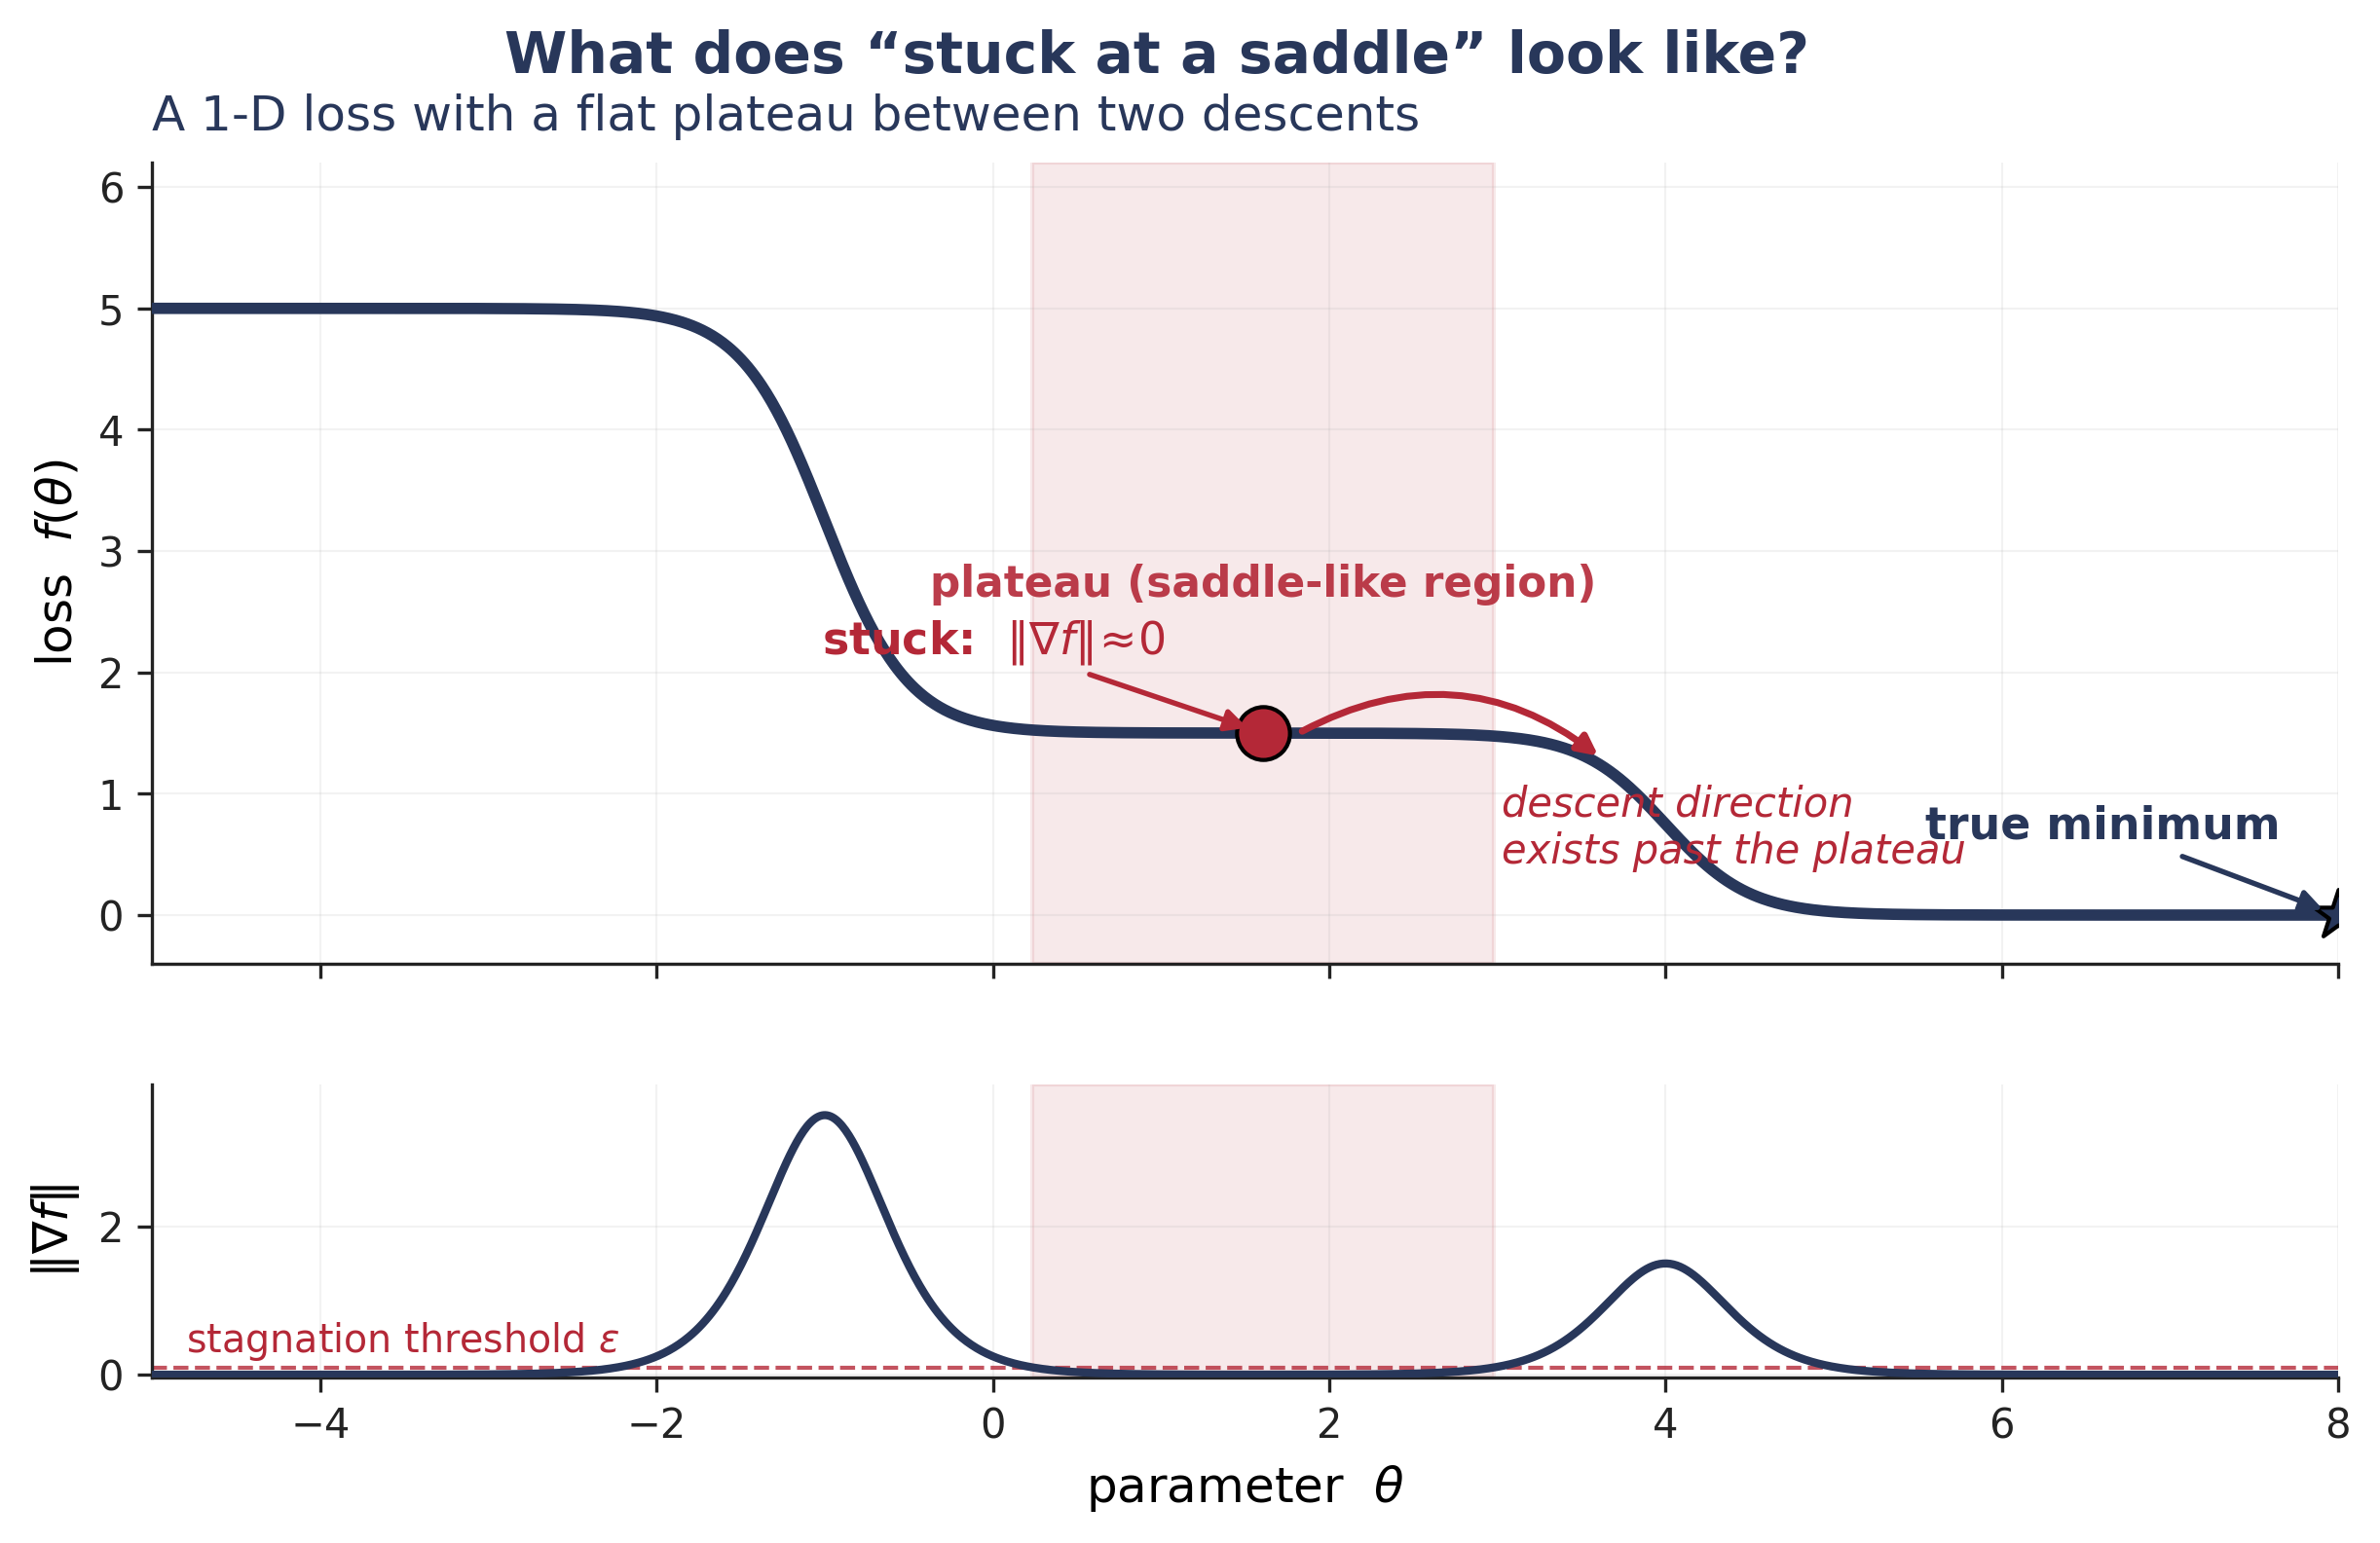
\includegraphics[width=\linewidth]{../figures/intuition_saddle_plateau.png}
  \end{columns}
\end{frame}

% ----- INTUITION 2: adaptive vs perturbation --- the core idea ------------
\begin{frame}{Two ways to get unstuck --- intuitively}
  \begin{block}{The hiking analogy}
    You're hiking down a foggy mountain to find the lowest valley.
    Sometimes the ground flattens out --- you're \emph{somewhere}, not
    at the bottom, and your sense of slope says ``stop.''
    Two strategies:
  \end{block}
  \vspace{0.3em}
  \begin{columns}[T,onlytextwidth]
    \column{0.48\textwidth}
      \begin{block}{Adaptive: \emph{walk smarter}}
        \footnotesize
        Don't just step in the gradient direction --- learn that some
        compass directions have always been flat (need bigger strides),
        and some have been steep (need smaller, careful steps).
        \\[0.4em]
        \alert{Adam, RMSProp, AdaGrad} do exactly this:
        rescale $\nabla f$ per-coordinate by past gradient
        magnitudes.\\[0.3em]
        \warn{Still only uses the loss at where you are right now.}
      \end{block}
    \column{0.48\textwidth}
      \begin{block}{Perturbation: \emph{take a leap}}
        \footnotesize
        When the slope tells you ``no progress,'' \emph{jump} a few
        feet in a random direction and check if you've fallen.
        Most jumps land you back on flat ground; some land you on
        a downhill slope.
        \\[0.4em]
        \alert{PGD} \scriptsize{\citep{jin2017escape}} \footnotesize injects
        Gaussian noise when the gradient gets small, then continues
        with gradient descent.
        \\[0.3em]
        \warn{Commits to the first jump regardless of where it lands.}
      \end{block}
  \end{columns}
\end{frame}

% ----- INTUITION 3: why perturbation works at all -------------------------
\begin{frame}{Why does ``take a leap'' actually work?}
  \begin{block}{The geometry behind it}
    \footnotesize
    A strict saddle has a ``tail'' --- directions of \emph{negative}
    curvature where the loss decreases. The gradient is zero
    \emph{exactly} at the saddle, so first-order methods see
    nothing.\\[0.4em]
    But: \alert{a random direction will, with positive probability,
    have a component along that tail}. Once you've nudged
    onto the tail, the gradient is again informative and you slide
    downhill.
  \end{block}
  \vspace{0.4em}
  \begin{itemize}\setlength\itemsep{0.3em}
    \item In 1-D: a flat plateau followed by a slope. Random jump
          left or right $\Rightarrow$ probability $\tfrac{1}{2}$
          you land on the slope.
    \item In high $d$: tail directions occupy a measure-positive
          fraction of the unit sphere; random isotropic noise hits
          one with overwhelming probability.
  \end{itemize}
  \vspace{0.4em}
  \pause
  \begin{block}{The remaining question}
    \centering
    \emph{Among the random jumps you could take, which one should
          you commit to?}\\
    \alert{This is precisely the gap SPGD fills.}
  \end{block}
\end{frame}

% ===========================================================================
% PART 2 -- WHAT IS SPGD
% ===========================================================================

\section{What is SPGD?}

% ----- INTUITION: SPGD as "look before you leap" --------------------------
\begin{frame}{SPGD, intuitively --- ``look before you leap''}
  \begin{block}{The one-line idea}
    \centering
    PGD takes \emph{one} random jump and hopes for the best.\\
    \alert{SPGD takes \np{} random jumps, and commits to the one that
           actually lowers the loss the most.}
  \end{block}

  \vspace{0.5em}
  \begin{columns}[T,onlytextwidth]
    \column{0.48\textwidth}
      \begin{block}{Why this should help}
        \footnotesize
        A single random jump might land you back on the plateau, or even
        \emph{up} the slope of the saddle's tail.\\[0.4em]
        Out of \np{} candidates, you're far more likely to find one
        that points to a genuinely lower loss --- and you only commit
        \alert{if} that minimum candidate actually beats your current
        position.
      \end{block}
    \column{0.48\textwidth}
      \begin{block}{Where SPGD sits between two extremes}
        \footnotesize
        \centering
        \begin{tabular}{r c l}
          Plain GD & $\longleftarrow$ \;\alert{SPGD}\; $\longrightarrow$ & Random search \\
          \scriptsize directed & & \scriptsize exploratory \\
          \scriptsize (no exploration) & & \scriptsize (no direction)
        \end{tabular}
        \\[0.4em]
        Directed efficiency of GD with the exploratory benefits of
        stochastic search.
      \end{block}
  \end{columns}

  \vspace{0.5em}
  \pause
  \centering
  \emph{Now the technical algorithm just makes this idea precise.}
\end{frame}

\begin{frame}{Now the precise version --- three differences from PGD}
  \scriptsize{\citep{vahedi2024spgd}}
  \vspace{0.4em}

  Three differences from PGD:
  \begin{enumerate}\setlength\itemsep{0.5em}
    \item \alert{When?} Perturbation fires \emph{unconditionally} every
          \iterp{} steps, not gated on stagnation detection. \\
          \scriptsize\emph{(PGD waits until $\|\nabla f\|$ is small;
          SPGD perturbs proactively.)}
    \item \alert{How many?} \np{} candidates per phase, not one. \\
          \scriptsize\emph{(PGD: single Gaussian sample.\;SPGD:
          \np{} uniform samples.)}
    \item \alert{Which one?} Commit the candidate with the steepest
          loss decrease (paper's $\le$ rule); else take the gradient step. \\
          \scriptsize\emph{(PGD has no selection step at all.)}
  \end{enumerate}
\end{frame}

\begin{frame}{The SPGD algorithm}
  \scriptsize
  \begin{algorithmic}[1]
    \Require initial \(\theta_0\), learning rate \(\eta\), amplitude \amp{},
             candidates \np{}, interval \iterp{}, total steps \(T\)
    \For{\(t = 0, \dots, T-1\)}
      \If{\(t \bmod \iterp{} = 0\) \textbf{and} \(t > 0\)}
        \State Sample \np{} candidates
               \(\delta^{(k)} \!\sim\! \mathrm{Uniform}(-\amp,\amp)^d\)
        \State Evaluate \(f(\theta_t + \delta^{(k)})\) for \(k = 1,\dots,\np{}\)
        \State \(k^\star \gets \arg\min_k f(\theta_t + \delta^{(k)})\)
        \If{\(f(\theta_t + \delta^{(k^\star)}) \le f(\theta_t)\)}
          \State \(\theta_t \gets \theta_t + \delta^{(k^\star)}\)
                 \quad\(\triangleright\) \textit{accept candidate (paper's $\le$ rule)}
        \EndIf
      \EndIf
      \State \(\theta_{t+1} \gets \theta_t - \eta\,\nabla f(\theta_t)\)
             \quad\(\triangleright\) \textit{standard gradient step}
    \EndFor
  \end{algorithmic}
  \vspace{0.5em}
  \normalsize
  \begin{itemize}
    \item Cost per perturbation phase: \np{} extra forward passes (no extra gradients).
    \item Hyperparameters that matter: \alert{\np{}} (exploration breadth) and
          \alert{\iterp{}} (exploration frequency).
  \end{itemize}
\end{frame}

% ===========================================================================
% PART 3 -- THE GAP IN THE LITERATURE
% ===========================================================================

\section{The Gap}

\begin{frame}{What did the original SPGD paper test?}
  \begin{columns}[T,onlytextwidth]
    \column{0.49\textwidth}
      \begin{block}{Tested on}
        \begin{itemize}
          \item 4 smooth 2-D benchmark functions \\
                (Peaks, Ackley, Easom, Levy~13)
          \item A 3-D component packing problem \\
                (NP-hard, mechanical engineering)
        \end{itemize}
      \end{block}
    \column{0.49\textwidth}
      \begin{block}{Compared against}
        \begin{itemize}
          \item Plain Gradient Descent (GD)
          \item PGD
          \item Simulated Annealing
          \item MATLAB \texttt{fmincon}
        \end{itemize}
      \end{block}
  \end{columns}

  \vspace{0.6em}
  \alert{What the paper does not include:}
  \begin{itemize}\setlength\itemsep{0.25em}
    \item Any neural-network experiment.
    \item Any same-compute random-selection control \\
          (so we cannot tell whether the \emph{selection rule} is what matters).
  \end{itemize}

  \pause
  \vspace{0.5em}
  \begin{block}{The paper's own future-work claim}
    ``\emph{Potential to significantly enhance neural network training}''
    \quad{\scriptsize\citep[Conclusion]{vahedi2024spgd}}
  \end{block}
  \centering
  \emph{This claim has not been tested. That is the gap we close.}
\end{frame}

\begin{frame}{Two questions only experiments can answer}
  \begin{block}{Q1 --- Does the paper's NN-training claim hold?}
    The authors say SPGD ``has potential'' on neural networks. Does it?
    Under what conditions, by how much?
  \end{block}

  \vspace{0.6em}
  \begin{block}{Q2 --- Is it the \emph{selection rule} or just the \emph{perturbation}?}
    SPGD's mechanism has two parts: \alert{multi-candidate perturbation}
    and \alert{steepest selection}. The original paper conflates them.
    We need a control that perturbs the same way but \emph{selects randomly}.
  \end{block}

  \vspace{0.4em}
  \pause
  \centering
  \emph{Our central methodological contribution is to introduce that control.}
\end{frame}

% ===========================================================================
% PART 4 -- METHODOLOGY
% ===========================================================================

\section{Methodology}

\begin{frame}{The five optimisers we compare}
  \small
  \begin{tabular}{>{\bfseries}l p{0.78\textwidth}}
    \toprule
    SGD  & Plain gradient descent. The first-order baseline. \\[0.2em]
    Adam & Per-parameter adaptive scaling. The modern ML default. \\[0.2em]
    PGD  & Gradient descent with one Gaussian perturbation when \(\|\nabla f\|\) is small. \\[0.2em]
    \alert{RPGD} & \alert{Random control:} same multi-candidate perturbation as SPGD, but commits a \emph{random} candidate (not the steepest). \\[0.2em]
    SPGD & Steepest of \np{} uniform candidates committed; paper's \(\le\) rule. \\
    \bottomrule
  \end{tabular}

  \vspace{0.7em}
  \begin{block}{What each contrast isolates}
    \begin{itemize}\setlength\itemsep{0.2em}
      \item SPGD vs.\ \alert{RPGD}: \,is the \emph{selection rule} doing useful work? \;(novel)
      \item SPGD vs.\ PGD: \,does multi-candidate perturbation help at all?
      \item SPGD vs.\ SGD: \,does perturbation+selection beat no perturbation?
    \end{itemize}
  \end{block}
\end{frame}

\begin{frame}{Paired-seed protocol + direct saddle diagnostics}
  \begin{columns}[T,onlytextwidth]
    \column{0.48\textwidth}
      \begin{block}{Paired-seed protocol}
        \small
        For each (experiment, seed):
        \begin{itemize}
          \item data split, init,
          \item all per-seed randomness
        \end{itemize}
        are fixed \emph{before} the optimiser is selected.\\[0.3em]
        All five optimisers run on \emph{identical} starting state.\\[0.3em]
        \alert{Differences are paired,} not unpaired.
      \end{block}
    \column{0.48\textwidth}
      \begin{block}{Direct saddle diagnostics}
        \small
        \begin{itemize}
          \item \emph{Stagnation episode}: max consecutive run with
                \(\|\nabla f\|_2 < \varepsilon\).
          \item \(\varepsilon = 10^{-4}\) on smooth benchmarks; \(10^{-3}\) on
                noisy mini-batches.
          \item \emph{Escape-time}: first step at which loss drops $5\%$
                below initial. Reported where saddle plateaus exist.
        \end{itemize}
      \end{block}
  \end{columns}
  \vspace{0.5em}
  \emph{We measure saddle behaviour directly --- not infer it from loss curves.}
\end{frame}

\begin{frame}{Six experiments (four discriminating, two diagnostic)}
  \small
  \begin{tabularx}{\textwidth}{>{\bfseries}l X r}
    \toprule
    \textbf{Exp} & \textbf{What it tests} & \textbf{Role} \\
    \midrule
    1 & Synthetic Rastrigin / Ackley / Rosenbrock at $d \in \{2,10,50\}$  & main \\
    3 & OpenML-CC18 tabular: 5 datasets, 3-layer MLP                       & main \\
    4 & \alert{CIFAR-10 / ResNet-18 anchor} (paired SPGD vs.\ RPGD)        & main \\
    6 & MovieLens-100K matrix completion (Burer--Monteiro)                 & main \\
    \midrule
    2 & Two Moons --- visualisation sanity check                           & appendix \\
    5 & $\np \times \iterp$ ablation                                       & appendix \\
    \bottomrule
  \end{tabularx}

  \vspace{0.7em}
  \emph{Increasing scale: $d=2$ \;$\to$\; $1.3{\times}10^{4}$ \;$\to$\;
        $1.1{\times}10^{7}$ parameters.}
\end{frame}

% ===========================================================================
% PART 5 -- EXPERIMENT WALKTHROUGH
% ===========================================================================

\section{Experimental Findings}

% --- EXP 1 ------------------------------------------------------------------
\begin{frame}{Experiment 1 --- Synthetic benchmarks}
  \begin{columns}[T,onlytextwidth]
    \column{0.47\textwidth}
      \footnotesize
      \textbf{Setup.}
      Rastrigin, Ackley, Rosenbrock; $d \in \{2,10,50\}$; 30 seeds per cell.
      Convergence: $f(\theta) < 10^{-2}$.
      \\[0.4em]
      \textbf{Findings.}
      \begin{itemize}\setlength\itemsep{0.15em}
        \item Cleanest signal on \alert{Ackley $d{=}10$:} SPGD's mean
              final loss is $-2.57$ below RPGD's (paired).
        \item At $d{=}50$ a \emph{constant} amplitude becomes destructive
              ($\sqrt{50/2}\!\approx\!5\times$ the displacement).
        \item Per-parameter scaling of \amp{} fixes this in subsequent experiments.
      \end{itemize}
    \column{0.5\textwidth}
      \centering
      
\includegraphics[width=\linewidth]{figures/exp1_success_rate.png}\\[0.2em]
      \scriptsize{Success rate per (function, dimension, optimiser).}
  \end{columns}
\end{frame}

% --- EXP 3 ------------------------------------------------------------------
\begin{frame}{Experiment 3 --- OpenML-CC18 tabular}
  \begin{columns}[T,onlytextwidth]
    \column{0.49\textwidth}
      \footnotesize
      \textbf{Setup.} 5 datasets (\texttt{credit-g}, \texttt{kc1},
      \texttt{spambase}, \texttt{segment}, \texttt{vehicle}), 3-layer MLP,
      3 seeds each.
      \\[0.4em]
      \textbf{Findings.}
      \begin{itemize}\setlength\itemsep{0.15em}
        \item SPGD's mean test accuracy above RPGD's on a majority of
              (dataset, seed) pairs.
        \item Adam dominates absolute accuracy on all 5 datasets ---
              tabular landscapes are well-conditioned.
        \item Stagnation rare; only \texttt{credit-g} and \texttt{vehicle}
              produced any non-zero counts.
      \end{itemize}
    \column{0.49\textwidth}
      \centering
      
\includegraphics[width=\linewidth]{figures/exp3_acc_per_dataset.png}\\[0.2em]
      \scriptsize{Test accuracy per dataset (mean $\pm$ 1 std, 3 seeds).}
  \end{columns}
\end{frame}

% --- EXP 4 (the headline) ---------------------------------------------------
\begin{frame}{Experiment 4 --- CIFAR-10 / ResNet-18 \;(\alert{anchor result})}
  \footnotesize
  \begin{columns}[T,onlytextwidth]
    \column{0.46\textwidth}
      \textbf{Setup.}
      ResNet-18 (11M params), BN disabled in \texttt{layer1}/\texttt{layer2}
      to retain saddle structure; 50 epochs, 3 seeds; $\amp{=}10^{-3}$,
      $\np{=}5$, $\iterp{=}200$. Run on the WPI Turing cluster (A30).\\[0.5em]

      \textbf{Final test accuracies (3 seeds).}
      \begin{tabular}{lc}
        \toprule
        Adam & $0.9015 \pm 0.014$ \\
        \alert{SPGD} & \alert{$0.8277 \pm 0.028$} \\
        SGD  & $0.8268 \pm 0.019$ \\
        PGD  & $0.8091 \pm 0.014$ \\
        \alert{RPGD} & \alert{$0.7899 \pm 0.046$} \\
        \bottomrule
      \end{tabular}
    \column{0.51\textwidth}
      \centering
      
\includegraphics[width=\linewidth]{figures/exp4_paired_spgd.png}\\[0.2em]
      \scriptsize{Per-seed paired deltas SPGD\,$-$\,RPGD and SPGD\,$-$\,SGD.}
  \end{columns}

  \vspace{0.4em}
  \begin{block}{Headline}
    \centering
    \alert{SPGD beats RPGD on all three seeds:} paired mean
    $+3.78$ pp test accuracy ($+4.42$, $+1.14$, $+5.77$).\\
    Cleanest evidence in the study that the \emph{selection rule} matters.
  \end{block}
\end{frame}

% --- EXP 6 (matrix completion) ----------------------------------------------
\begin{frame}{Experiment 6 --- MovieLens matrix completion (saddle escape)}
  \footnotesize
  \begin{columns}[T,onlytextwidth]
    \column{0.46\textwidth}
      \textbf{Why this benchmark.}
      Burer--Monteiro factorisation of a $943\!\times\!1682$ rating matrix at
      rank 5, init $\mathcal{N}(0, 0.01^2)$. Documented saddle near origin
      that gradient descent escapes only slowly
      \scriptsize{\citep{ge2016matrix, sun2018geometric}}.

      \vspace{0.4em}
      \normalsize\textbf{The two key numbers.}\footnotesize
      \begin{itemize}\setlength\itemsep{0.15em}
        \item \alert{Acceptance rate}: SPGD fires at $30\!\pm\!2\%$;
              RPGD at $9\!\pm\!1\%$ \;($3{\times}$).
              \\\emph{The selection rule is empirically active.}
        \item \alert{Escape-time} (first $5\%$ loss drop):
              \begin{tabular}{l@{\;\;}l}
                SPGD$-$SGD  & $-50$ steps (3/3 seeds) \\
                SPGD$-$RPGD & $-40$ steps (3/3 seeds) \\
              \end{tabular}
      \end{itemize}

    \column{0.51\textwidth}
      \centering
      
\includegraphics[width=\linewidth]{figures/exp6_mc_curves.png}\\[0.2em]
      \scriptsize{Train MSE (left) and test RMSE (right). SPGD leads SGD
                  through the saddle, lead consumed by convergence.}
  \end{columns}

  \vspace{0.3em}
  \begin{block}{The split result}
    \alert{Mechanism transfers} (SPGD fires as designed in $d{\approx}13{,}000$),
    but the optimisation lead does \alert{not} translate into a held-out RMSE
    gap (paired $\Delta = -0.002$, sign mixed).\\
    \emph{Mechanism-positive, generalisation-neutral.}
  \end{block}
\end{frame}

% ===========================================================================
% PART 6 -- WHAT WE LEARNED
% ===========================================================================

\section{Synthesis}

\begin{frame}{Cross-experiment summary}
  \footnotesize
  \begin{tabular}{>{\bfseries}l c c c l}
    \toprule
    \textbf{Setting} & \textbf{SPGD vs.\ RPGD} & \textbf{Stagnation?} &
    \textbf{Effect size} & \textbf{Read} \\
    \midrule
    Synthetic ($d{=}10$, Ackley) & SPGD $\downarrow$ & yes & paired $-2.57$ loss & rule helps \\
    OpenML tabular               & SPGD slightly ahead & rare & $\sim$1 pp acc & rule helps \\
    \alert{CIFAR-10 / ResNet-18} & \alert{SPGD $>$ RPGD on 3/3} & \alert{none} & \alert{$+3.78$ pp} & \alert{rule helps strongly} \\
    MovieLens MC                 & training: SPGD $\downarrow$ & yes (saddle) & escape $-50$ steps & rule fires \\
    \bottomrule
  \end{tabular}

  \vspace{0.7em}
  \begin{block}{Headline result, one line}
    Across the four discriminating experiments, the
    \alert{steepest-selection rule} provides a measurable advantage over
    same-mechanism random perturbation.
  \end{block}

  \pause
  \vspace{0.4em}
  \emph{The advantage is mechanism-positive on every setting,\\
        and generalisation-positive on CIFAR-10 specifically.}
\end{frame}

\begin{frame}{Where the algorithm \emph{doesn't} help}
  \begin{block}{1.\;The saddle-escape framing is over-stated for modern ML}
    \alert{Zero stagnation episodes} ($\|\nabla f\|<10^{-3}$ for $\geq5$ steps)
    on \emph{all 15 CIFAR-10 runs}, despite our deliberately disabling BN in
    the early layers to preserve saddle structure. SPGD's CIFAR-10 advantage
    therefore cannot be attributed to plateau escape per se.
  \end{block}

  \vspace{0.4em}
  \begin{block}{2.\;Generalisation gain on matrix completion is null}
    SPGD's training-time lead on MovieLens does not survive to held-out
    RMSE (paired $\Delta = -0.002$, sign mixed across seeds).
  \end{block}

  \vspace{0.4em}
  \begin{block}{3.\;Adam dominates absolute accuracy throughout}
    Per-parameter adaptive scaling implicitly conditions the loss landscape;
    none of our perturbation methods rescale the gradient. The right
    comparison is therefore SPGD vs.\ same-compute random control,
    not SPGD vs.\ Adam.
  \end{block}
\end{frame}

% ===========================================================================
% PART 7 -- COMPARISON WITH ORIGINAL PAPER
% ===========================================================================

\section{Comparison with the Original Paper}

\begin{frame}{What did we add over the original SPGD paper?}
  \footnotesize
  \begin{tabular}{>{\bfseries}l p{0.34\textwidth} p{0.34\textwidth}}
    \toprule
     & \textbf{Original (Vahedi \& Ilies, 2024)} & \textbf{This work} \\
    \midrule
    Domain     & 2-D test functions, 3-D engineering packing &
                 Neural networks \& matrix completion \\
    Compared with & GD, PGD, SA, \texttt{fmincon} &
                 SGD, Adam, PGD, \alert{RPGD}, SPGD \\
    Random control? & \alert{absent} & \alert{introduced (RPGD)} \\
    Saddle diagnostic & inferred from loss curves &
                 \alert{stagnation episodes + escape-time} \\
    Paired protocol & no & \alert{yes (across all experiments)} \\
    Compute scale & seconds, 2-D & up to ResNet-18 / CIFAR-10 \\
    \bottomrule
  \end{tabular}

  \vspace{0.7em}
  \begin{block}{Bottom line}
    The original paper proposes the algorithm; we provide the first
    \alert{controlled, paired, ML-scale} test of its central claim
    --- and the only same-compute random-selection ablation in the literature.
  \end{block}
\end{frame}

\begin{frame}{Three things this study contributes}
  \begin{enumerate}\setlength\itemsep{0.45em}
    \item \alert{The first ML-scale test of SPGD.}\\
          The original paper names neural-network training as an
          in-scope use case (\emph{``unconstrained problems such as
          2-D test function benchmarks and neural network training\dots''})
          but reports no NN experiment. Our four discriminating
          experiments span synthetic, tabular, vision, and matrix
          completion at up to $1.1{\times}10^{7}$ parameters.
    \item \alert{An RPGD control that isolates the selection rule.}\\
          Without a same-compute random-selection baseline, ``SPGD
          beats baselines'' is confounded with ``perturbation alone
          helps.'' On CIFAR-10/ResNet-18 the SPGD-vs-RPGD paired delta
          is $+3.78$~pp on every seed; that gap could not have been
          measured by the original protocol.
    \item \alert{Bounded scope claims, supported by direct diagnostics.}\\
          Stagnation episodes and escape-time give us measurements,
          not assertions: the algorithm helps where the selection rule
          fires (CIFAR-10, $d{=}10$ Ackley), and is neutral where it
          doesn't transfer to held-out loss (MovieLens RMSE).
  \end{enumerate}
\end{frame}

% ===========================================================================
% PART 8 -- CONCLUSION
% ===========================================================================

\section{Conclusion}

\begin{frame}{What we conclude}
  \begin{block}{Main empirical claim}
    On modern ML loss landscapes, SPGD's value is best framed as a
    \alert{biased candidate-selection rule}, not a saddle-escape mechanism.
  \end{block}

  \vspace{0.4em}
  \begin{block}{Methodological recommendation}
    \alert{Future perturbation-based optimisers should be benchmarked
    against a same-compute random-selection control}, a comparison
    missing from the existing literature. On our deepest setting it is
    the selection \emph{rule}, not perturbation alone, that does the
    useful work.
  \end{block}

  \vspace{0.4em}
  \begin{block}{One-line take-away}
    \centering
    \emph{It's not the noise. It's the choice.}
  \end{block}
\end{frame}

\begin{frame}{Limitations (briefly)}
  \footnotesize
  \begin{itemize}\setlength\itemsep{0.3em}
    \item Three seeds at the CIFAR-10 scale --- mitigated by paired protocol
          but unpaired stds are wide.
    \item Stagnation threshold $\varepsilon$ is fixed; a relative threshold
          might surface plateaus our absolute one misses.
    \item No momentum / lr-schedule on SPGD --- adaptivity held out to
          isolate the selection rule.
    \item Constant amplitude \amp{}; per-parameter scaling
          $\amp_p \propto \mathrm{std}(\theta_p^{(0)})$ would likely improve
          $d{=}50$ and ResNet-18.
    \item Flat-minima / sharpness measurement scoped out (zero-stagnation
          made it peripheral here).
  \end{itemize}
\end{frame}

\begin{frame}[plain]
  \centering
  \vspace{1.5em}
  {\Huge\bfseries\color{slateblue} Thank you.}\\[1.5em]
  {\Large Questions?}\\[2em]
  {\small
   \emph{Repository} \quad\(\rightarrow\)\quad
   \url{https://github.com/shyampatadia/spgd_research}\\[0.4em]
   \emph{Code, configs, and figures} \quad\(\rightarrow\)\quad
   \texttt{src/spgd\_study/}, \texttt{experiments/}, \texttt{figures/}.\\[0.3em]
   \emph{Numerical artefacts} \quad\(\rightarrow\)\quad
   \texttt{results/exp6\_escape\_time\_paired.json} (escape-time deltas).
  }
\end{frame}

% ===========================================================================
% BACKUP SLIDES (will follow the "Thank you" slide; useful for Q\&A)
% ===========================================================================

\appendix

\section*{Backup}

\begin{frame}{Backup --- Why $\varepsilon = 10^{-3}$ on noisy gradients?}
  \footnotesize
  \begin{itemize}\setlength\itemsep{0.3em}
    \item On smooth full-batch losses (Exp 1, Two Moons), gradient norms
          decay smoothly to $O(10^{-4})$ near minima; we use the
          proposal's $\varepsilon = 10^{-4}$.
    \item On mini-batched CIFAR-10/OpenML, the gradient-norm time series
          is dominated by mini-batch noise --- typical norms are
          $O(10^{-2})$. A $10^{-4}$ threshold would never fire.
    \item We pick $10^{-3}$ as the consistent ``well below typical
          mini-batch noise floor'' threshold.
    \item The \emph{qualitative} CIFAR-10 result (zero stagnation) is
          threshold-dependent; we flag this as a limitation.
  \end{itemize}
\end{frame}

\begin{frame}{Backup --- $\np \times \iterp$ ablation (appendix)}
  \begin{columns}[T,onlytextwidth]
    \column{0.32\textwidth}
      \footnotesize
      \begin{itemize}\setlength\itemsep{0.2em}
        \item Grid: $\np\!\in\!\{1,5,10,20\}$, $\iterp\!\in\!\{5,10,50,100\}$.
        \item 80 runs (5 seeds$\times$16 cells), Two Moons, $\sim$2~min total.
        \item Compute scales $\propto\!\np\!/\!\iterp$, range $\sim\!400\times$.
        \item Accuracy heatmap mostly flat: SPGD is robust to hyper choice.
        \item Loss heatmap: smaller \iterp{} reaches lower loss without
              accuracy gain $\Rightarrow$ broader basins, not deeper ones.
      \end{itemize}
    \column{0.66\textwidth}
      \centering
      
\includegraphics[width=\linewidth]{figures/exp5_heatmap_acc.png}
  \end{columns}
\end{frame}

\begin{frame}{Backup --- Two Moons trajectories (appendix)}
  \centering
  
\includegraphics[width=0.96\linewidth]{figures/exp2_loss_landscape.png}\\[0.3em]
  \footnotesize
  Shared PCA basis: PC1, PC2 mean the same in every panel; $\theta_0$ at the origin.
  Adam moves substantially along PC1 (adaptive directions);
  SGD/PGD/RPGD/SPGD all move predominantly along PC2.\\
  \emph{Diagnostic of geometry, not a benchmark of accuracy.}
\end{frame}

\begin{frame}{Backup --- Bibliography (selected)}
  \footnotesize
  \begin{thebibliography}{99}
    \bibitem{vahedi2024spgd}
      A. M. Vahedi, H. T. Ilies. ``SPGD: Steepest Perturbed Gradient
      Descent Optimization,'' \emph{arXiv:2411.04946}, 2024.
    \bibitem{jin2017escape}
      C. Jin, R. Ge, P. Netrapalli, S. M. Kakade, M. I. Jordan.
      ``How to Escape Saddle Points Efficiently,'' \emph{ICML}, 2017.
    \bibitem{ge2015escaping}
      R. Ge, F. Huang, C. Jin, Y. Yuan. ``Escaping from saddle points,''
      \emph{COLT}, 2015.
    \bibitem{dauphin2014saddle}
      Y. Dauphin et al. ``Identifying and attacking the saddle point
      problem in high-dimensional non-convex optimization,''
      \emph{NeurIPS}, 2014.
    \bibitem{ge2016matrix}
      R. Ge, J. D. Lee, T. Ma. ``Matrix completion has no spurious local
      minimum,'' \emph{NeurIPS}, 2016.
    \bibitem{sun2018geometric}
      J. Sun et al. ``A geometric analysis of phase retrieval and
      related problems.'' 2018.
    \bibitem{he2016resnet}
      K. He, X. Zhang, S. Ren, J. Sun. ``Deep residual learning for image
      recognition,'' \emph{CVPR}, 2016.
    \bibitem{kingma2015adam}
      D. Kingma, J. Ba. ``Adam: A method for stochastic optimization,''
      \emph{ICLR}, 2015.
  \end{thebibliography}
\end{frame}

\end{document}
